\begin{figure}[htbp]
    \begin{subfigure}{.5\textwidth}
    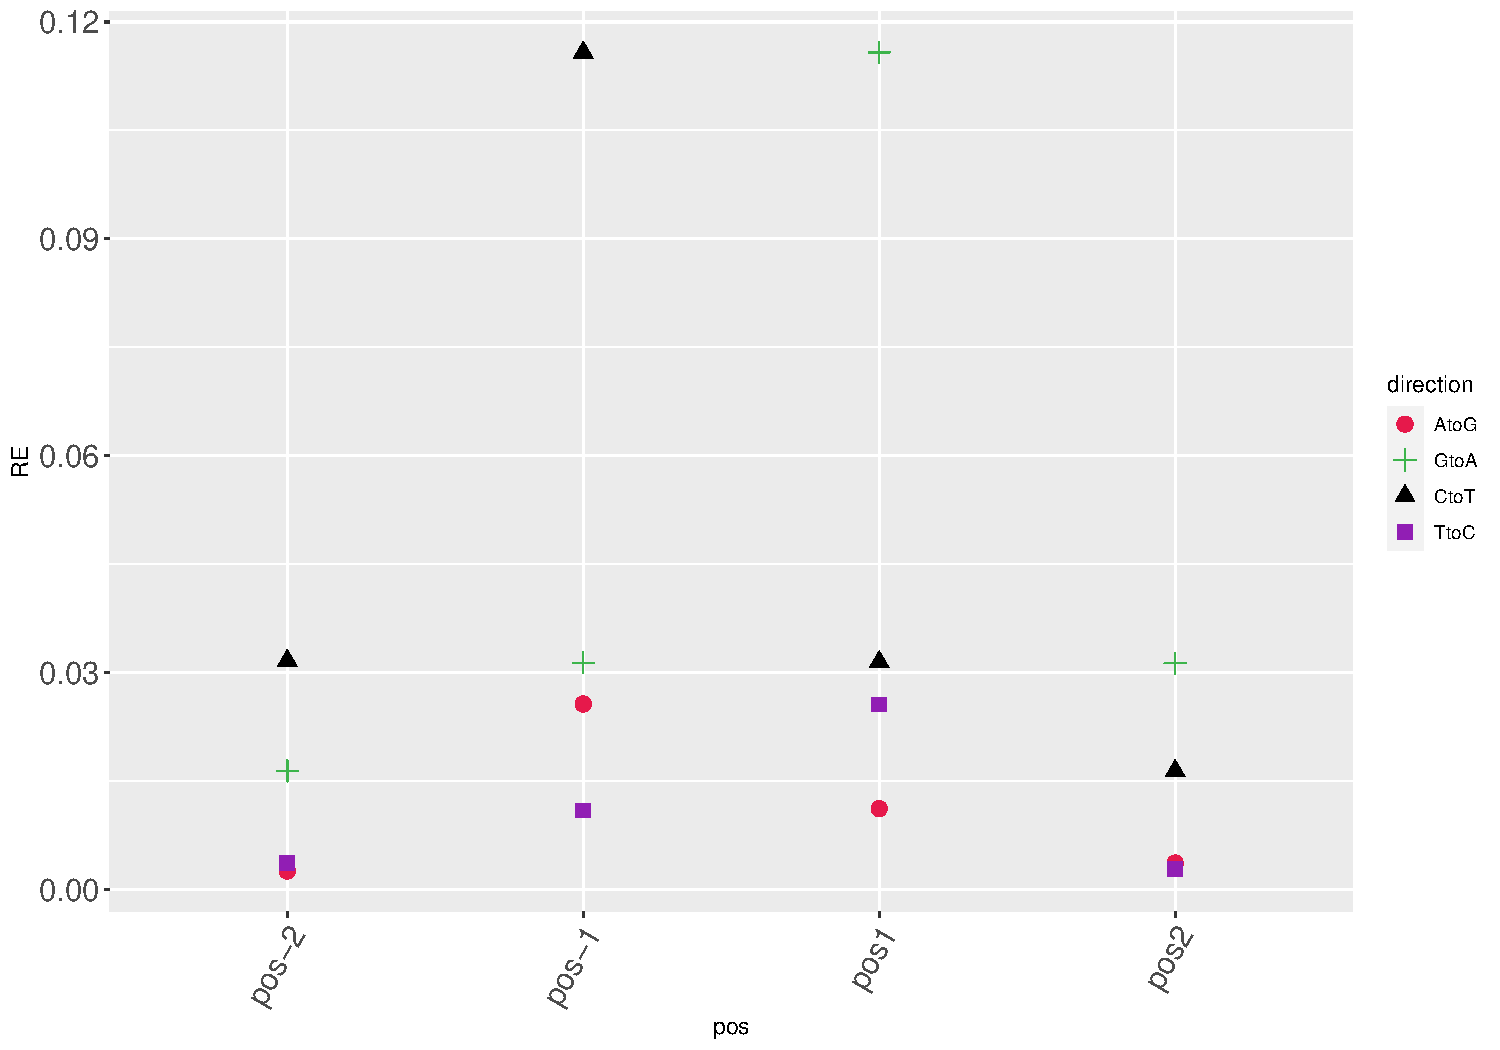
\includegraphics[scale=0.7]{graphics/nbr_transitions_Skin-Melanoma.pdf}
    \caption{transitions/Skin-Melanoma}
    \label{fig:transitions_skin}
    \end{subfigure}
    ~
    \begin{subfigure}{.5\textwidth}
    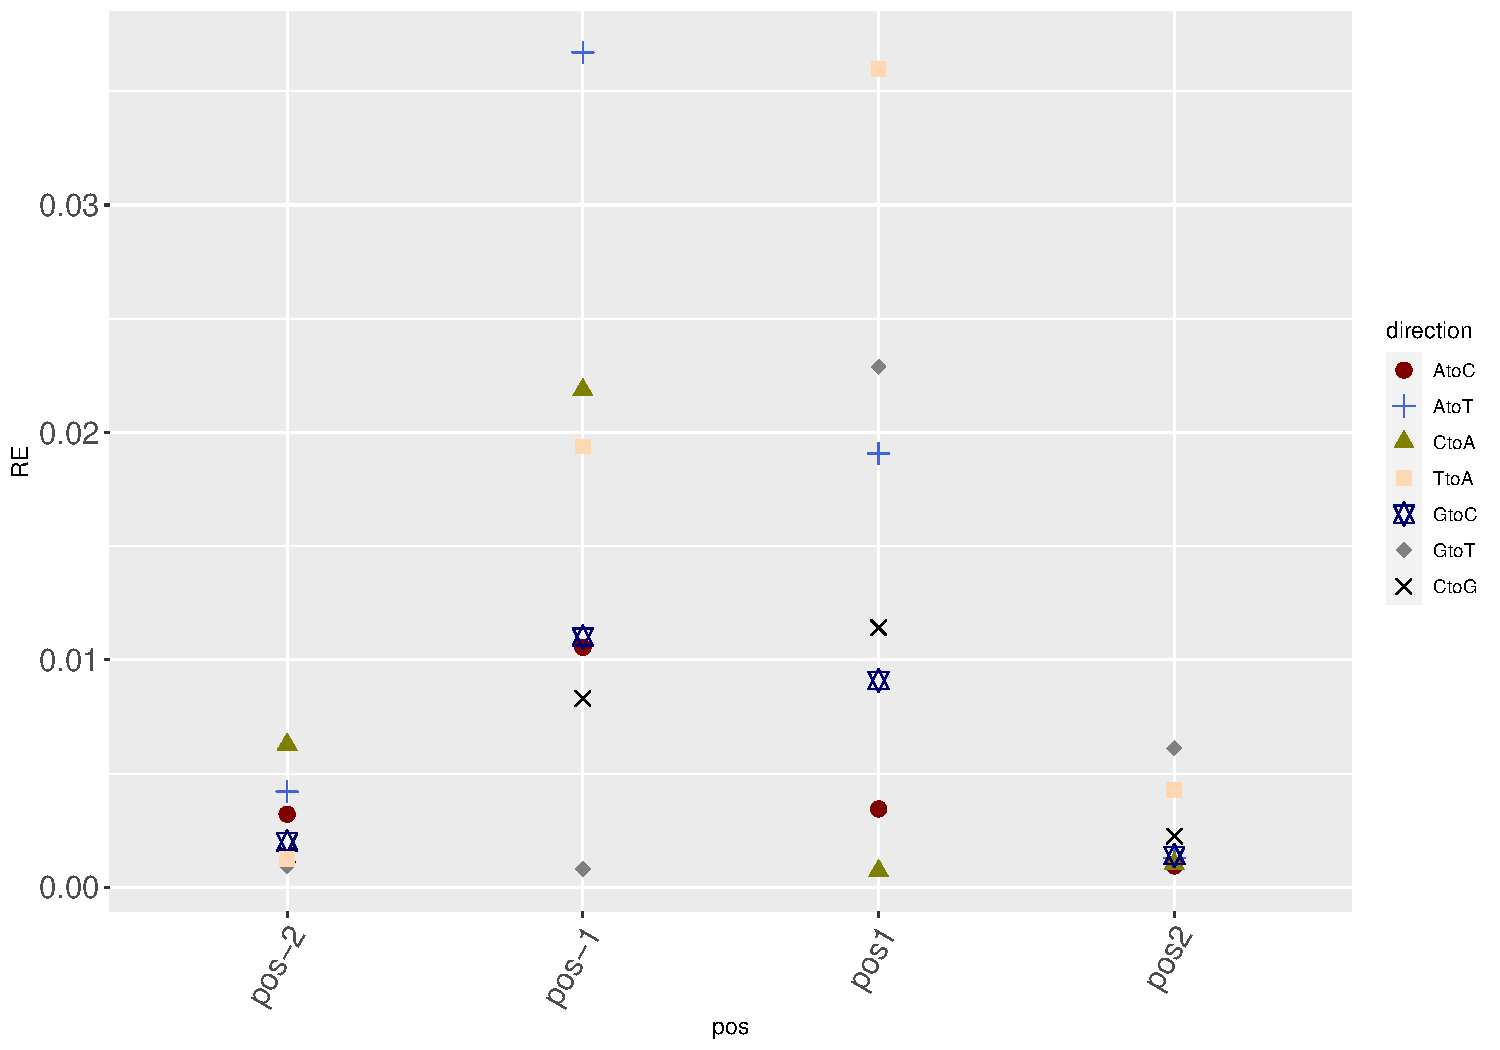
\includegraphics[scale=0.7]{graphics/nbr_transversion_Skin-Melanoma.pdf}
    \caption{transversions/Skin-Melanoma}
    \label{fig:transversions_skin}
    \end{subfigure} \\
    \vspace{0.5cm}
    
    \begin{subfigure}{.5\textwidth}
    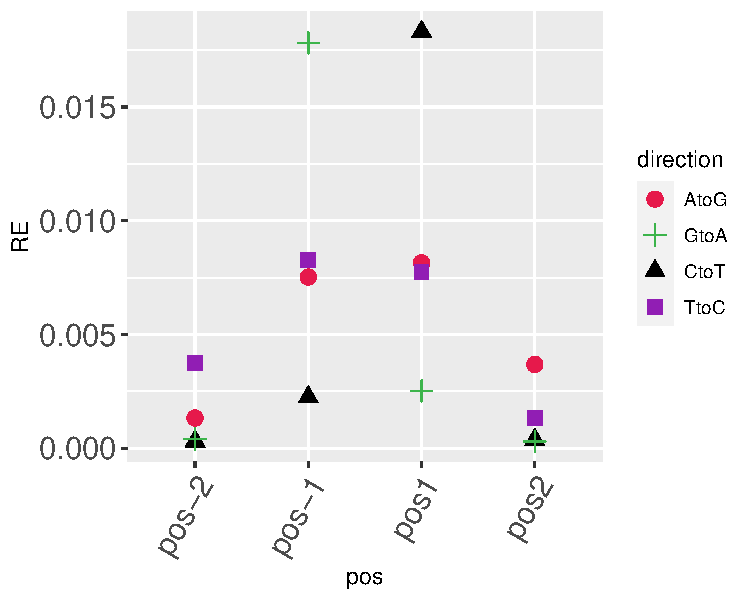
\includegraphics[scale=0.7]{graphics/nbr_transitions_Liver-HCC.pdf}
    \caption{transitions/Liver-HCC}
    \label{fig:transitions_liver}
    \end{subfigure}
    ~
    \begin{subfigure}{.5\textwidth}
    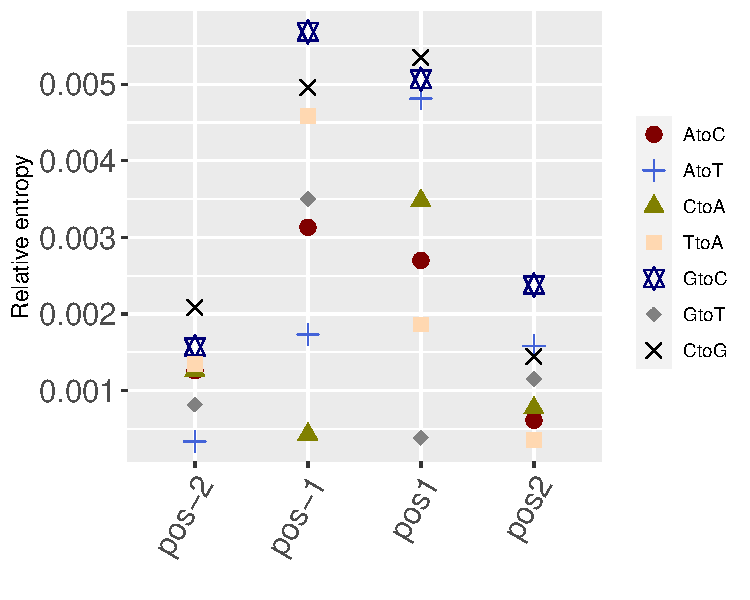
\includegraphics[scale=0.7]{graphics/nbr_transversion_Liver-HCC.pdf}
    \caption{transversion/Liver-HCC}
    \label{fig:transversion_liver}
    \end{subfigure} \\
    
    \caption{\textbf{Base substitutions are a rich source of information, manifested by $RE$}. Here, $RE$'s are shown in sequence logos for (a) Skin-Melanoma (b) Kidney-RCC (c) Liver-HCC (d) Panc-AdenoCA. For each panel, each row was derived from a GLM. The x-axis is the wildtype base; the y-axis is the product of the substitution. The heights of the letters are $RE$'s. An up-orientation indicates an excess while a down-orientation indicates a deficit of the mutation.}
    \label{fig:nbr}
\end{figure}